% cap3.tex

\chapter{Methodology}
\label{ch:metodo} % la etiqueta para referencias

\color{blue}{} En esta sección de debe incluir el diseño experimental y metodología general del trabajo que fueron utilizados, su explicación, así como el detalle de los materiales, equipos y metodologías teóricas y experimentales utilizadas. (Máximo 15 páginas). }


\section{Ejemplo de texto}
In this section, we outline the process of collecting the necessary data for our research, which included both Chilean and international legal corpora, as well as projects from the Chilean SEA 

For each model, a JSON structure is created to store all the metrics for each epoch during the fine-tuning process. This structure allows for easy tracking and analysis of the model's performance on different datasets. Each model that is fine-tuned on a specific dataset has its unique JSON file containing the corresponding metrics. The JSON structure captures various metrics that assess the performance of the model on the task of environmental impact assessment, an example of this JSON can be seen in figure 3.3. These metrics include:

\vspace{0.5cm}
\begin{figure}[H]
\label{fig:JSON Fine Tune Stago}
\centering
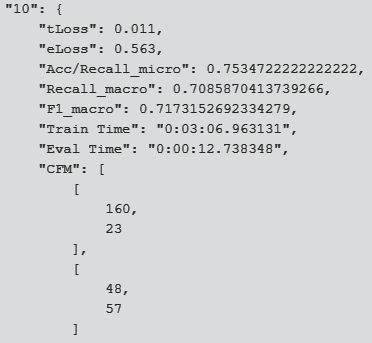
\includegraphics[scale=0.5]{images/JSON_ft.png}
\caption[Example JSON created during fine-tuning]{Example JSON created during fine-tuning, Source: Self-Made}
\end{figure}

\begin{itemize}
   \item 10: This number corresponds to the fine-tunning epoch.
   \item tLoss (Training Loss): The training loss value at the last epoch indicates how well the model learned from the training data.
   \item eLoss (Evaluation Loss): The evaluation loss value at the last epoch represents the loss on the evaluation data, providing insights into the model's generalization ability.
   \item Acc/Recall micro (Accuracy/Recall - Micro Average): This metric represents the micro-average accuracy and recall, which provide an overall measure of the model's performance across all classes.
   \item Recall macro (Recall - Macro Average): The macro-average recall calculates the average recall across all classes, providing a measure of the model's performance for individual classes.
   \item F1 macro (F1 Score - Macro Average): The macro-average F1 score calculates the average F1 score across all classes, considering both precision and recall.
   \item Train Time: The training time for the last epoch, indicating the duration required to train the model on the dataset.
   \item Eval Time: The evaluation time for the last epoch, representing the time taken to evaluate the model's performance on the dataset.
   \item Confusion Matrix (CFM): The confusion matrix provides detailed information about the model's performance for each class, showing the number of true positive, false positive, true negative, and false negative predictions.
 \end{itemize}

By storing these metrics in a structured JSON format, it becomes easier to analyze the performance of the fine-tuned models and compare their results across different epochs and datasets. The confusion matrix is also graphed using a heat map for easier understanding and comparing, Figure 3.4 shows the final confusion matrix.

\vspace{0.5cm}
\begin{figure}[H]
\label{fig:Confusion Matrix Example}
\centering
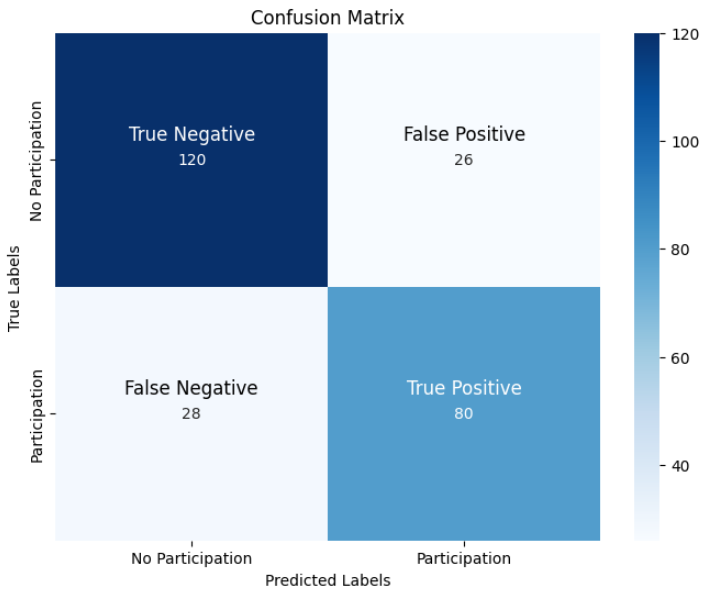
\includegraphics[scale=0.8]{images/Example_CM.png}
\caption[Confusion Matrix Example]{Confusion Matrix Example, Source: Self-Made}
\end{figure}